\documentclass[a4paper, 12pt]{article}
\usepackage[a4paper,top=1.5cm, bottom=1.5cm, left=1cm, right=1cm]{geometry}
\usepackage[utf8]{inputenc}
\usepackage{mathtext}
\usepackage{amsmath}
\usepackage{amsfonts}
\usepackage[english, russian]{babel}
\usepackage{indentfirst}
\usepackage{longtable}
\usepackage{graphicx}
\graphicspath{{pictures/}}
\DeclareGraphicsExtensions{.pdf,.png,.jpg}
\usepackage{natbib}
\usepackage{hyperref}
\usepackage{emoji}
\babelfont{rm}{Droid Serif}
\babelfont{sf}{Droid Sans}
\renewcommand{\baselinestretch}{1.3}
\usepackage{wrapfig}

\title{Решение задачи брахистохроны}
\author{Платонов Егор и Николаев Михаил}
\date{\today}

\begin{document}

\maketitle
\section{Постановка проблемы}
Проблемой данной задачи является нахождение кривой между двумя точками с заданными координатами, спуск тела по которой без начальной скорости в однородном поле тяжести займет наименьшее время. Такая кривая называется брахистохроной. В данной работе пренебрежено воздействием на тело силы трения и силы сопротивления воздуха.
\section{Вывод уравнения брахистохроны}
\subsection{Вывод зависимости времени спуска от траектории}
Введём систему координат XOY (рис. \ref{xoy}) начало которой находится в начальной точке спуска, а ось абсцисс сонаправлена с вектором ускорения свободного падения $\overrightarrow{g}$ конечная точка спуска будет иметь координаты $(\Delta x; \Delta y)$. В этой системе отсчета будут проводиться все дальнейшие вычисления.
\begin{figure}[h]
    \centering
    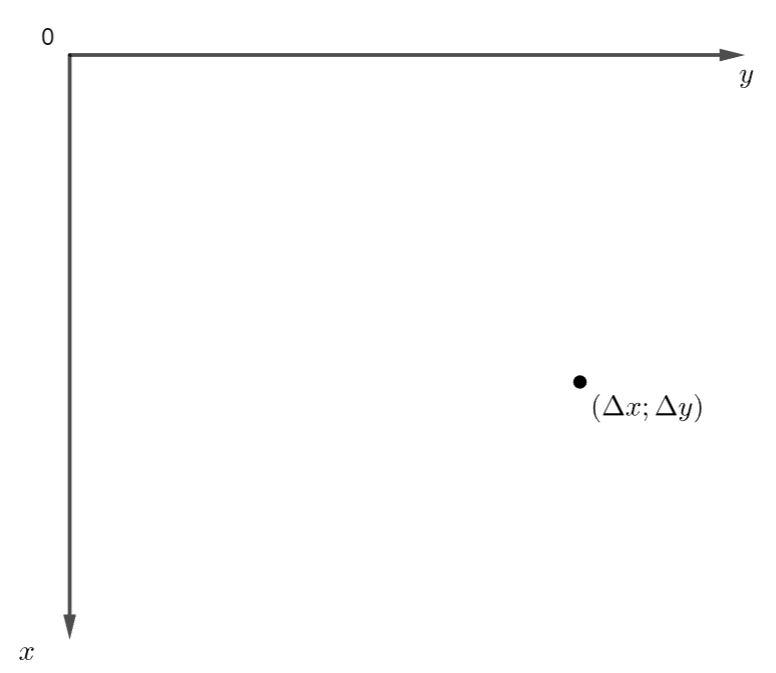
\includegraphics[width=250pt]{xoy.png}
    \caption{Система координат XOY}
    \label{xoy}
\end{figure}

Воспользуемся законом сохранения энергии, чтобы выразить скорость спуска тела на определенной выcоте:
\[ v = \sqrt{2gx}\]
Выразим приращение длины дуги:
\begin{equation}
    ds = \sqrt{(dx)^2+(dy)^2} = \sqrt{1+(y'(x))^2} dx
    \label{ds}
\end{equation}
Приращение времени это приращение пути поделённое на скорость:
\[ dt = \frac{ds}{v} = \frac{\sqrt{1+(y'(x))^2} dx}{\sqrt{2gx}} = \frac{1}{2g} \sqrt{\frac{1+(y'(x))^2}{x}}dx\]
Проинтегрируем $dt$, чтобы получить полное время спуска t:

\begin{equation}
    t = \frac{1}{2g} \int_{0}^{\Delta x} \sqrt{\frac{1+(y'(x))^2}{x}} \,dx
\end{equation}

Чтобы решить задачу нужно найти такую фунцию $y(x)$, при которой интеграл t принимает наименьшее значение, для этого потребуется составить уравнение Эйлера-Лагранжа. Сформулируем уравнение Эйлера-Лагранжа.
\subsection{Формулировка Уравнения Эйлера-Лагранжа}
Пусть задан функционал $J(f)$:

\[ J(f) = \int_{a}^{b} F(x, f(x), f'(x)) \,dx\]
на пространстве гладких функций $f:[a,b] \rightarrow \mathbb{R}$, где через $f'$ обозначена первая производная $f$ по $x$.

Предположим, что подынтегральная функция $F(x, f(x), f'(x))$, дважды непрерывно дифференцируема.
Если функционал $J$ достигает экстремума на некоторой функции $f$, то для неё должно выполняться обыкновенное дифференциальное уравнение (уравнение Эйлера-Лагранжа):

\[ \frac{\partial F}{\partial y} - \frac{d}{dx} \left( \frac{\partial F}{\partial y'} \right) = 0 \]

, где знаком $\partial$ обозначается частная производная (производная функции нескольких переменной по одной из них, при неизменных остальных переменных).
\subsection{Решение дифференциального уравнения}
Составим уравнение Эйлера-Лагранжа для фунционала $t$. Поскольку $t$ не зависит от $y(x)$, член $\frac{\partial F}{\partial y}$ равен нулю.


\[ \frac{\partial F}{\partial y'} = \frac{y'(x)}{\sqrt{x(1+(y'(x))^2)}} \]

\[ \frac{d}{dx} \left( \frac{y'(x)}{\sqrt{x(1+(y'(x))^2)}} \right) = 0 \]

Из чего следует:

\[ \frac{y'(x)}{\sqrt{x(1+(y'(x))^2)}} = c, \]
где $c$ - константа, отличная от нуля

С учетом (\ref{ds}):

\begin{equation}
    \frac{dy}{ds} = c\sqrt{x}
    \label{dy/ds}
\end{equation}

С геометрической точки зрения:

\begin{equation}
    \frac{dx}{ds} = cos(\varphi), \frac{dy}{ds} = sin(\varphi),
    \label{dx/ds dy/ds}
\end{equation}
где $\varphi$ -- угол между касательной к траектории и положительным направлением оси абсциссс.
Из (\ref{dy/ds}) и (\ref{dx/ds dy/ds}) следует:
\begin{equation}
    x = \frac{\sin^2\varphi}{c^2}
    \label{x}
\end{equation}

Из (\ref{dx/ds dy/ds}) и (\ref{x}) следует:

\begin{equation}
    \frac{dy}{d\varphi} = \frac{dy}{dx}\cdot\frac{dx}{d\varphi} = \tg\varphi \frac{dx}{d\varphi}=\tg\varphi\frac{d}{d\varphi}\left( \frac{\sin^2\varphi}{c^2} \right) = 2\frac{\sin^2\varphi}{c^2},
\end{equation}
откуда

\begin{equation}
    y = \frac{2}{c^2}(2\varphi-\sin2\varphi)
    \label{y}
\end{equation}

В (\ref{x}) и (\ref{y}) заменим $2/c^2$ на $R$, a $2\varphi$ на t:
\begin{equation}
    x = R(1-\cos t)
\end{equation}

\begin{equation}
    y = R(t-\sin t)+b
    \label{yc}
\end{equation}
Если подставить в (\ref{yc}) точку (0; 0), то получится, что $b=0$

Конечные уравнения выглядят так:

\begin{equation}
    x = R(1-\cos t)
\end{equation}

\begin{equation}
    y = R(t-\sin t)
\end{equation}

Если представить, что $R$ -- радиус колеса, катящегося без проскальзывания по плоской поверхности, а $t$ -- это угол его поворота, то станет очевидно, что x(y) изображает циклоиду (рис. \ref{cycloid}) -- траекторию которую описывает точка на ободе колеса, катящегося по плоской поверхности без проскальзывания.

\begin{figure}[ht!]
    \centering
    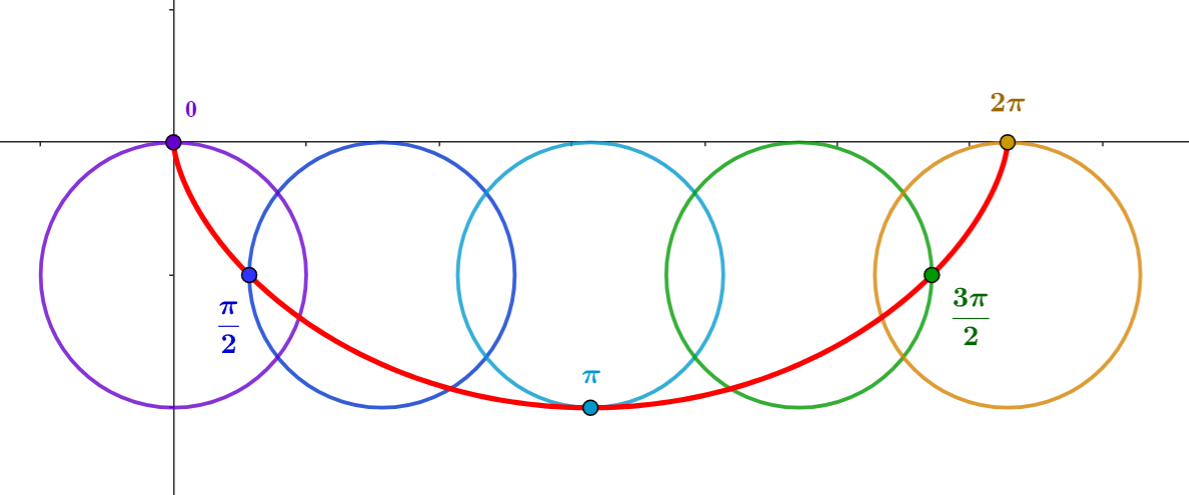
\includegraphics[width = 450pt]{cycloid.png}
    \caption{Циклоида}
    \label{cycloid}
\end{figure}

\end{document}